\documentclass[11pt]{article}

% Paquetes
%===============================================================================

% Establecemos los márgenes
\usepackage[a4paper, margin=1in]{geometry}

% Separacion entre parrafos
\setlength{\parskip}{1em}

% Paquete para incluir codigo
\usepackage{listings}
\usepackage{listings-rust}

% Paquete para incluir imagenes
\usepackage{graphicx}
\graphicspath{ {./images/} }

% Para fijar las imagenes en la posicion deseada
\usepackage{float}

% Para que el codigo acepte caracteres en utf8
\lstset{literate=
  {á}{{\'a}}1 {é}{{\'e}}1 {í}{{\'i}}1 {ó}{{\'o}}1 {ú}{{\'u}}1
  {Á}{{\'A}}1 {É}{{\'E}}1 {Í}{{\'I}}1 {Ó}{{\'O}}1 {Ú}{{\'U}}1
  {à}{{\`a}}1 {è}{{\`e}}1 {ì}{{\`i}}1 {ò}{{\`o}}1 {ù}{{\`u}}1
  {À}{{\`A}}1 {È}{{\'E}}1 {Ì}{{\`I}}1 {Ò}{{\`O}}1 {Ù}{{\`U}}1
  {ä}{{\"a}}1 {ë}{{\"e}}1 {ï}{{\"i}}1 {ö}{{\"o}}1 {ü}{{\"u}}1
  {Ä}{{\"A}}1 {Ë}{{\"E}}1 {Ï}{{\"I}}1 {Ö}{{\"O}}1 {Ü}{{\"U}}1
  {â}{{\^a}}1 {ê}{{\^e}}1 {î}{{\^i}}1 {ô}{{\^o}}1 {û}{{\^u}}1
  {Â}{{\^A}}1 {Ê}{{\^E}}1 {Î}{{\^I}}1 {Ô}{{\^O}}1 {Û}{{\^U}}1
  {ã}{{\~a}}1 {ẽ}{{\~e}}1 {ĩ}{{\~i}}1 {õ}{{\~o}}1 {ũ}{{\~u}}1
  {Ã}{{\~A}}1 {Ẽ}{{\~E}}1 {Ĩ}{{\~I}}1 {Õ}{{\~O}}1 {Ũ}{{\~U}}1
  {œ}{{\oe}}1 {Œ}{{\OE}}1 {æ}{{\ae}}1 {Æ}{{\AE}}1 {ß}{{\ss}}1
  {ű}{{\H{u}}}1 {Ű}{{\H{U}}}1 {ő}{{\H{o}}}1 {Ő}{{\H{O}}}1
  {ç}{{\c c}}1 {Ç}{{\c C}}1 {ø}{{\o}}1 {å}{{\r a}}1 {Å}{{\r A}}1
  {€}{{\euro}}1 {£}{{\pounds}}1 {«}{{\guillemotleft}}1
  {»}{{\guillemotright}}1 {ñ}{{\~n}}1 {Ñ}{{\~N}}1 {¿}{{?`}}1 {¡}{{!`}}1
}

% Para que no se salgan las lineas de codigo
\lstset{breaklines=true}

% Para que los metadatos que escribe latex esten en español
\usepackage[spanish]{babel}

% Para la bibliografia
% Sin esto, los enlaces de la bibliografia dan un error de compilacion
\usepackage{url}

% Para mostrar graficas de dos imagenes, cada una con su caption, y con un caption comun
\usepackage{subcaption}

% Simbolo de los numeros reales
\usepackage{amssymb}

% Para que los codigos tengan una fuente distinta
\usepackage{courier}

\lstdefinestyle{CustomStyle}{
  language=Python,
  numbers=left,
  stepnumber=1,
  numbersep=10pt,
  tabsize=4,
  showspaces=false,
  showstringspaces=false
  basicstyle=\tiny\ttfamily,
}

% Para incluir tablas en csv
\usepackage{csvsimple}

% Para referenciar secciones usando el nombre de las secciones
\usepackage{nameref}

% Para enumerados dentro de enumerados
\usepackage{enumitem}

% Mostrar la página de las referencias en el indice del documento
\usepackage[nottoc,numbib]{tocbibind}

% Metadatos del documento
%===============================================================================
\title{
{Práctica 3b}\\
{Búsqueda por Trayectorias}\\
{Problema de Agrupamiento con Restricciones}\\
}
\author{
{Sergio Quijano Rey - 72103503k}\\
{4º Doble Grado Ingeniería Informática y Matemáticas}\\
{Grupo de prácticas 2 - Viernes 17.30h a 19.30h}\\
{sergioquijano@correo.ugr.es}
}
\date{\today}

% Contenidos del documento
%===============================================================================

\begin{document}

% Portada del documento
\maketitle
\pagebreak

% % Indice de contenidos
\tableofcontents

% Lista de figuras
\listoffigures

\pagebreak

\section{Descripción del problema}

Vamos a trabajar el problema del agrupamiento con restricciones (\textbf{\emph{PAR}}). Consiste en una generalización del problema de agrupamiento clásico, al que añadimos restricciones sobre los datos.

El problema de agrupamiento clásico consiste en, dados unos datos de entrada sin etiquetar $X$ de tamaño $n$, agruparlos en $k$ grupos (o en inglés, \emph{clusters}) diferentes, formando una partición $C$ de $X$, de forma que se optimice alguna métrica. Normalmente, se busca minimizar la distancia \emph{intra\_cluster} (que más tarde se definirá).

La diferencia con el problema de agrupamiento clásico, por tanto, es la inclusión de restricciones. En nuestro caso concreto, trabajemos con restricciones entre pares de puntos, que además serán de dos tipos:

\begin{itemize}
\item Restricción tipo \emph{Must Link}: los dos puntos afectados por esta restricción deberán pertenecer al mismo cluster
\item Restricción tipo \emph{Cannot Link}: los dos puntos afectados por esta restricción no deben pertenecer al mismo cluster
\end{itemize}

Consideraremos de forma débil estas restricciones, es decir, podemos incumplir algunas restricciones. Pero supondrá que la solución será de peor calidad. Para especificar mejor esta noción, definimos la función de \emph{fitness} que buscamos minimizar:

\begin{displaymath}
fitness(sol) := distancia_{intra-cluster}(sol) + \lambda * infeasibility(sol)
\end{displaymath}

donde $infeasibility$ es el número de restricciones que se incumplen. Esta función de $fitness$ nos permite pasar de intentar optimizar dos funciones objetivo a solo tener que optimizar un objetivo. El valor de $\lambda$ se especifica más adelante.

Como los datos no están etiquetados a priori, podríamos considerar este problema como un problema de aprendizaje no supervisado. Sin embargo, se puede considerar que las restricciones nos dan un tipo de etiquetado, por lo que es más correcto pensar que estamos ante una tarea de aprendizaje \emph{semi-supervisado}. La principal utilidad de resolver estos problemas es que normalmente estamos reduciendo la dimensionalidad de los datos a analizar, y de este modo, es más sencillo extraer conocimiento sobre dichos datos.

\pagebreak

\section{Descripción de la aplicación de los algoritmos empleados}

\subsection{Representación del conjunto de datos}

Los datos vienen dados en una matriz de tamaño $n \times d$ donde $n$ es el número de puntos y $d$ es la dimensión de cada uno de los puntos.

\subsubsection{Representación del conjunto de datos en código}

El conjunto de datos viene representado en \lstinline{problem_datatypes::DataPoints} que contiene un vector de otro tipo de dato: \lstinline{problem_datatypes::Point}. El tipo de dato \lstinline{Point} tiene un campo que es de tipo \lstinline{ndarray::Array1<f64>} que representa un vector (usamos una librería para trabajar con matrices y vectores). Por tanto, hemos pasado de trabajar con una matriz de datos a trabajar con un vector de puntos. Esto nos permite trabajar de forma más expresiva y sencilla con el problema. Por ejemplo, podemos calcular con métodos del \lstinline{struct} distancia entre dos puntos, centroide de un conjunto de puntos, \ldots

\subsection{Representación de las restricciones}

Las restricciones vienen dadas en un fichero de datos que representa una matriz que codifica las restricciones de la siguiente forma:

\begin{itemize}
\item El elemento en la fila $i$-ésima y columna $j$-ésima representa las restricciones que hay entre el punto $i$ y el punto $j$
\item Como la restricción que tenga el punto $i$ con el punto $j$ implica que el punto $j$ tiene la misma restricción con el punto $i$, es claro que dicha matriz debe ser simétrica
\item Un valor $0$ significa que no hay restricciones. Un valor $1$ significa que hay una restricción tipo \emph{Must Link}. Un valor $-1$ implica una restricción \emph{Cannot Link}
\item Además, la matriz tiene la diagonal de $1$s
\end{itemize}

\subsubsection{Representación de las restricciones en código}

El \lstinline{struct} \lstinline{problem_datatypes::Constraints} junto al enumerado \lstinline{problem_datatypes::ConstraintType} representan en el código las restricciones. El código es el siguiente:

\begin{lstlisting}[language=Rust, style=Boxed]
pub enum ConstraintType {
MustLink,
CannotLink,
}

pub struct Constraints{
data: HashMap<(i32, i32), ConstraintType>,
}
\end{lstlisting}

Es claro que guardamos pares de enteros, que marcan los índices de los puntos, y la restricción entre el par de puntos representados, en un \lstinline{HashMap}. Esta elección viene motivada por:

\begin{itemize}
\item Podemos acceder a las restricciones entre dos puntos en tiempo constante
\item Podemos iterar sobre todas las restricciones, gracias a los métodos proporcionados por el lenguaje de programación, en un tiempo más que razonable. Así iteramos solo sobre una lista de $r$ restricciones, en vez de sobre una matriz cuadrada de dimensión $n^2$
\item En cierto modo, estamos combinando los beneficios de tener acceso directo a elementos concretos y los beneficios de poder iterar sobre una lista (aunque iterar sobre un \lstinline{Hash} puede ser algo más lento que iterar sobre una lista o un \lstinline{array})
\item Es fácil de implementar métodos para operar con restricciones con este tipo de dato
\end{itemize}

La implementación de los métodos que permiten manipular el \lstinline{struct} aseguran que:
\begin{itemize}
\item No guardamos la restricción $(i, j)$ y junto a la $(j, i)$. Solo guardamos una de las dos restricciones, ahorrando memoria
\item De hecho, el criterio es guardar como índices el par $(i, j)$ donde $i \leq j$
\item Tampoco guardamos las restricciones $(i, i), MustLink$ pues son restricciones triviales
\end{itemize}


\subsection{Representación de la solución}

Una representación de la solución será un vector de tamaño $n$ con valores en $\{0, \ldots, k - 1\}$ donde $n$ es el número de puntos y $k$ es el número de clusters en los que dividimos los datos. Este vector representa la partición de los datos en los $k$ clusters. En la posición $i$-ésima del vector, guardamos el cluster al que pertenece el punto $i$-ésimo de nuestro conjunto de datos.

Las soluciones deben cumplir las siguientes restricciones:

\begin{itemize}
\item No pueden quedar clusters vacíos. Es decir, clusters a los que no haya ningún punto asignado. Esto puede verse viendo que $\forall i \in \{0, \ldots, k-1\}$ $\exists pos \in \{0, \ldots, n-1\}$ tal que $solution[pos] = i$, es decir, el vector de soluciones tiene al menos una vez cada valor posible de los clusters
\item Cada punto solo puede pertenecer a un único cluster. Por la forma vectorial en la que representamos la partición, esta restricción se verifica forzosamente, y por tanto no nos tenemos que preocupar de realizar comprobaciones
\item La unión de los puntos de los clusters debe ser todo el conjunto de datos, es decir, $X = \bigcup c_i$. De nuevo, nuestra representación vectorial fuerza a que esta restricción se verifique
\end{itemize}

Por ejemplo, si tenemos 5 puntos y 3 clusters, una posible solución sería $\{3, 1, 2, 3, 0\}$. Y por otro lado, la solución $\{3, 1, 2, 3, 2\}$ no es válida pues el cluster $0$ está vacío.

Para cada solución podemos calcular algunas métricas necesarias para conocer el valor de $fitness$ de la solución que estamos representando. Para comenzar, por cada cluster podemos calcular el \textbf{centroide} del cluster:

\begin{displaymath}
\vec{\mu_i} := \frac{1}{|c_i|} \sum_{x_i \in c_i} \vec{x_i}
\end{displaymath}

Definimos para cada cluster su \textbf{distancia media intra-cluster} como:

\begin{displaymath}
\bar{c_i} := \frac{1}{|c_i|} \sum_{x_i \in c_i} || \vec{x_i} - \vec{\mu_i} ||_2
\end{displaymath}

Y con ello podemos definir la \textbf{desviación general de la partición} como:

\begin{displaymath}
\bar{c} := \frac{1}{k} \sum_{i \in 1, \ldots k} \bar{c_i}
\end{displaymath}

Definimos $infeasibility$ como el número de restricciones, tanto del tipo \emph{Must Link} como del tipo \emph{Cannot Link}, que se violan.

Con ello, ya podemos definir el valor de $\lambda$ como $\lambda := \frac{D}{|R|}$ donde $|R|$ es el número total de restricciones y $D$ la distancia máxima entre dos puntos de $X$.

Cuando trabajemos con algoritmos poblacionales, usaremos la siguiente \textbf{nomenclatura}:

\begin{itemize}
    \item Población: conjunto de soluciones
    \item Cromosoma: una solución individual
    \item Gen: cada uno de los elementos del vector de asignación punto $\rightarrow$ cluster que compone la solución
\end{itemize}

\subsubsection{Representación de la solución en código}

La solución se representa en la clase \lstinline{problem_datatypes::Solution}. El código de los campos del \lstinline{struct} desarrollado es:

\begin{lstlisting}[language=Rust, style=Boxed]
pub struct Solution<'a, 'b> {
cluster_indexes: Vec<u32>,
data_points: &'a DataPoints,
constraints: &'b Constraints,
number_of_clusters: i32,

/// Representa el peso de infeasibility en el calculo de fitness
/// Solo se calcula una vez al invocar a Solution::new
lambda: f64,

// Para cachear el valor de fitness pues es un calculo costoso de realizar
// Como los datos del struct no cambian, podemos hacer el cacheo sin miedo
// Usamos RefCell para tener un patron de mutabilidad interior
fitness: RefCell<Option<f64>>,
}
\end{lstlisting}

Los campos del \lstinline{struct} representan:

\begin{itemize}
\item \lstinline{cluster_indixes}: el vector solución que representa la asignación de puntos a clusters
\item \lstinline{data_points}: referencia al conjunto de datos (sirve para calcular métricas como el $fitness$ de la solución que se representa)
\item \lstinline{constraints}: referencia al conjunto de restricciones sobre los datos (sirve para calcular métricas como el $fitness$ de la solución que se representa)
\item \lstinline{number_of_clusters}: número de clusters en los que se agrupan los datos (sirve para comprobar que una solución sea válida)
\item \lstinline{lambda}: valor de $\lambda$, necesario para calcular el $fitness$
\item \lstinline{fitness}: valor de $fitness$. Está incluida en un \lstinline{RefCell<Option<f64>>} para poder cachear su valor, puesto que los atributos de una instancia nunca cambian y el cálculo del valor $\lambda$ es muy costoso (implica calcular restricciones violadas y distancias entre puntos)
\end{itemize}

La comprobación de que no tenemos clusters sin puntos asignados se hace en el método \lstinline{Solution::is_valid}. La distancia media intracluster se calcula en \lstinline{Solution::intra_cluster_distance}. Mientras que la desviación general se calcula en \lstinline{Solution::global_cluster_mean_distance}. El valor de $infeasibility$ se calcula en \lstinline{Solution::infeasibility}. El cálculo de $\lambda$ se realiza en el \emph{constructor} del \lstinline{struct}.

Además, en todos los algoritmos, salvo \lstinline{copkmeans}, debemos llevar la cuenta de las evaluaciones de \emph{fitness} que consumimos. Para ello tenemos la función \lstinline{fitness_and_consumed}. También tenemos funciones para invalidar la cache, para comprobar si tenemos el \emph{fitness} cacheado o no, $\ldots$

\subsubsection{FitnessEvaluationResult}

Para mejorar el control sobre las evaluaciones del fitness, disponemos del struct  \lstinline{FitnessEvaluationResult<T>}. Guarda un tipo genérico \lstinline{T} y las evaluaciones que consume la operación que genera dicho valor. Por ejemplo, si en un población (de la que hablaremos más adelante), queremos encontrar el individuo con mejor valor de fitness, devolvemos \lstinline{FitnessEvaluationResult<Solution>} con dicho mejor individuo y las consumiciones de fitness \textbf{efectivas} que consume esta búsqueda.

\subsection{Representación de la población}

Una población, intuitivamente, es un conjunto de individuos, que en nuestro caso, serán soluciones válidas del problema que estamos intentando resolver. En código la representaremos como un vector de \lstinline{Solution}. Sobre este \lstinline{struct} podemos realizar operaciones comunes a los algoritmos genéticos, tanto generacionales como estacionarios, y a los algoritmos meméticos. Operaciones como generar una población inicial aleatoria, mutar con cierta probabilidad a la población, realizar  torneos binarios para generar una población de selección de tamaño dado, $\ldots$

\subsubsection{Representación en código y consideraciones}

El \lstinline{struct} viene dado por:

\begin{lstlisting}[language=Rust, style=Boxed]
/// Representa una poblacion para los algoritmos geneticos
#[derive(Debug, Clone)]
pub struct Population<'a, 'b>{
    /// Individuos de la poblacion
    individuals: Vec<Solution<'a, 'b> >,
}
\end{lstlisting}

Los métodos implementados para el \lstinline{struct} serán comentados a medida que vayamos describiendo el pseudocódigo de los distintos algoritmos.

Una consideración importante es que, en un primer momento, consideramos utilizar una estructura de datos del tipo \emph{Cola con prioridad}. De esta forma, podríamos obtener de forma eficiente los elementos mejores y peores (respecto a su valor del \emph{fitness}) de una población. Sin embargo, introducía mucha complejidad en el código, pues era difícil tener en cuenta las evaluaciones del fitness que se consumían al mantener la estructura de datos (por ejemplo, deberíamos haber implementado la interfaz \emph{Ord}, que no permite devolver el tipo de dato \emph{FitnessEvaluationResult}). Esto, junto a que el código corre en unos tiempos muy razonables, motiva nuestra decisión a no considerar una estructura de datos más compleja. Podría haber sido interesante implementar a mano un \lstinline{PriorityQueue} para poder controlar las evaluaciones del fitness y también optimizar algo más el código.

En los pseudocódigos mostramos que, en la función \lstinline{select_best_indixes}, usamos una cola con prioridad. Esto porque previamente evaluamos toda la población, y con ello, tenemos controladas las evaluaciones del fitness.

Notar también que muchos de los métodos devuelven el tipo \lstinline{FitnessEvaluationResult}, para tener control de las evaluaciones del fitness consumidas, como ya hemos comentado previamente.

\pagebreak

\section{Descripción de los algoritmos empleados}

\subsection{Búsqueda Local} \label{pseudocodigo_localsearch}

Usamos un pseudocódigo muy parecido a \lstinline{Python} pues es muy expresivo y facilita traducir partes de nuestro código real a pseudocódigo.

Método de exploración de entorno:

\begin{lstlisting}[language=Python, style=Boxed]
# Estrategia el primero mejor
# Devuelve el primer vecino que mejora la solucion actual
def get_neighbour():
    # Tomamos el generador de vecinos que se describe mas adelante
    neighbours_generator = generate_all_neighbours()

    # Mezclo los generadores de vecinos
    neighbours_generator.shuffle()

    # Exploro los vecinos hasta encontrar uno mejor que esta solucion
    for current_generator in neighbours_generator:
        current_solution = self.generate_solution_from(current_generator)

        if
            current_solution.is_valid() and
            current_solution.fitness() < self.fitness():

            return current_solution

    # No hemos encontrado un vecino mejor
    return None;
}
\end{lstlisting}

Operador de generación de vecino:

\begin{lstlisting}[language=Python, style=Boxed]

# Struct que representa el generador de vecinos de
# forma eficiente
struct NeighbourGenerator:
    # El elemento que queremos mover de cluster
    element_index: i32,

    # El nuevo cluster al que asignamos el elemento
    new_cluster: u32,

# Funcion que genera todos los vecinos posibles de un elemento
# Los vecinos generados pueden ser no validos
def generate_all_neighbours(
    number_of_elements,
    number_of_clusters):
    neighbours = []

    for current_element in 0..number_of_elements:
        for current_cluster in 0..number_of_clusters:
            neighbours.append(NeighbourGenerator{
                current_element,
                current_cluster,
            });

    return neighbours;
\end{lstlisting}

Generación de soluciones aleatorias:

\begin{lstlisting}[language=Python, style=Boxed]
# Genera una solucion inicial aleatoria como punto de partida de las busquedas
# Puede dejar clusters vacios, por lo que el caller de esta funcion tiene que
# comprobar la validez de la solucion aleatoria, y en caso de invalidez, volver
# a llamar a esta funcion (es muy poco probable que con muchos puntos dejemos
# un cluster vacio)
def generate_random_solution(data_points, constraints, number_of_clusters):
        # Vector con indices de clusters aleatorios, de tamaño el numero de puntos
        # que trabajamos
        random_cluster_indixes = [
            random(0, number_of_clusters)
            for _ in data_points.len()
        ]

        # En nuestro codigo, generamos el struct Solution a partir de los parametros
        # de entrada y random_cluster_indixes
        return solution_from(cluster_indexes)
    }
\end{lstlisting}


\pagebreak

\subsection{Descripción y Pseudocódigo del algoritmos de comparación - \emph{Copkmeans}}

Como algoritmo de comparación estamos considerando una modificación del algoritmo clásico \emph{K-means} al que añadimos la capacidad de considerar las restricciones: \emph{copkmeans} o \emph{Constrained K-means}. Por tanto, estamos ante un algoritmo \emph{greedy}.

La idea general es:

\begin{enumerate}
    \item Partir de una solución inicial aleatoria, que vendrá dada por una asignación de centroides de clusters aleatorios
    \item Iterar sobre todos los datos en orden aleatorio, asignando a cada punto el mejor cluster en ese momento (siguiendo claramente un esquema greedy). Consideramos como mejor cluster el que menos restricciones violadas produzca, y en caso de empate, el cluster cuyo centroide sea más cercano al punto
    \item Una vez acabada la asignación de todos los puntos, calcular los centroides de los clusters con la asignación actual de los puntos
    \item Repetir el proceso desde 2. si los centroides han cambiado respecto de la anterior iteración
\end{enumerate}

A la hora de ejecutar el algoritmo, en algunos \emph{datasets} el algoritmo se encuentra con problemas, pues los centroides pueden oscilar infinitamente entre dos soluciones muy cercanas (debido entre otros factores a la configuración de los datos de entrada). Esta configuración de los datos también puede provocar que haya clusters que se queden sin puntos asignados, generando así una solución no válida. Por tanto, el algoritmo admite un parámetro de entrada para indicar si queremos que sea \emph{robusto} o no. En caso de que indiquemos que queremos que sea robusto se tendrán las siguientes diferencias:

\begin{itemize}
    \item Los centroides aleatorios no se tomarán como puntos aleatorios, sino como puntos del \emph{dataset} aleatorios, por lo que en una primera iteración no podrán quedar clusters vacíos, aunque si podrán quedar clusters vacíos en iteraciones posteriores. Con esto se buscas evitar el problema de los clusters vacíos
    \item Se tendrá un máximo de iteraciones. Este máximo lo hemos establecido como 50 iteraciones sobre el bucle principal. Teniendo en cuenta que cuando no cicla infinitamente, en menos de 10 iteraciones el algoritmo encuentra solución, consideramos que es un máximo mucho más que aceptable para asegurar que la solución devuelta sea la mejor (o la segunda mejor) que el \emph{greedy} puede calcular con esa semilla aleatoria. Con esto se busca evitar el problema del ciclado infinito
    \item Aún con estos cambios, en ciertas ocasiones no podemos evitar que dejemos un cluster vacío en iteraciones posteriores a la primera. Por tanto, también colocaremos un máximo de reinicios del algoritmo en la parte del código que llama al método de búsqueda.
\end{itemize}

El pseudocódigo (en notación muy parecida a \lstinline{Python}) de nuestra implementación del algoritmo quedaría tal que:

\begin{lstlisting}[language=Python, style=Boxed]
# Generamos los centroides aleatorios. Dependiendo de si es robust o no
# consideramos puntos aleatorios en [0,1] x [0,1] o puntos del dataset
# de entrada aleatorios
current_centroids = generate_random_centroids()

# Solucion inicial aleatoria que se va a modificar en la primera iteracion
# Notar que no es valida porque deja todos los clusters menos uno vacíos
current_cluster_indixes = [0, 0, ..., 0]

# Para comprobar que los centroides cambien
centroids_have_changed = true


# Si robust == true, acotamos el numero maximo de iteraciones
max_iterations = 50
mut curr_iteration = 0

while centroids_have_changed == true and curr_iteration < max_iterations{

    # Realizamos una nueva asignacion de clusters. Recorremos los puntos
    # aleatoriamente y asignamos el cluster que menos restricciones viole
    # en esa iteracion. En caso de empate, se toma el cluster con centroide
    # mas cercano al punto
    new_cluster_indixes = assign_points_to_clusters()

    # Comprobamos que la nueva solucion calculada es correcta
    if valid_cluster_configuration(current_cluster_indixes) == false:
        # Esto hace que el el caller de la funcion copkmeans, se muestre un
        # mensaje por pantalla y se vuelva a realizar la busqueda, con lo que
        # partimos de unos centroides aleatorios nuevos. Como ya se ha comentado,
        # hay un maximo de reinicios en el caller para este metodo
        return None

    # Calculamos los nuevos centroides y comprobamos si han cambiado
    new_centroids = calculate_new_centroids(new_cluster_indixes)
    centroids_have_changed = centroids_are_different(
        current_centroids,
        new_centroids
    )

    # Cambiamos a la nueva asignacion de clusters y los nuevos centroides
    current_cluster_indixes = new_cluster_indixes
    current_centroids = new_centroids


    # En caso de que robust = true, acotamos el numero de iteraciones de forma
    # efectiva aumentando el contador. En otro caso, al no tocar el contador
    # no estamos teniendo en cuenta este parametro
    if robust == true:
        curr_iteration = curr_iteration + 1;

# Devolvemos la solucion en la estructura de datos correspondiente
return solution_from(current_cluster_indixes)
\end{lstlisting}

Desarrollamos el código de \lstinline{assign_points_to_clusters} por su importancia:

\begin{lstlisting}[language=Python, style=Boxed]
def assign_points_to_clusters():
    # Realizamos una nueva asignacion de clusters
    # -1 para saber que puntos todavia no han sido asignados a un cluster
    new_cluster_indixes= [-1, -1, ..., -1]

    # Recorremos aleatoriamente los puntos para irlos asignando a cada cluster
    point_indexes = (0..data_points.len())
    point_indexes.shuffle();

    for index in point_indexes:
        # Calculo el cluster al que asignamos el punto actual
        new_cluster_indixes[index] = select_best_cluster(
            current_cluster_indixes,
            current_centroids,
        )

    # Devolvemos los indices que representan la solucion
    return new_cluster_indixes
\end{lstlisting}

\pagebreak

\subsection{Descripción y pseudocódigo del algoritmo de búsqueda local multiarranque básica}

Este algoritmo consiste en lanzar, con distintas soluciones iniciales aleatorias, la búsqueda local fuerte implementada en la práctica 1. Tras lanzar el número dado de veces esta búsqueda local, nos quedamos con la solución que mejor \emph{fitness} ha alcanzado. En \emph{\ref{pseudocodigo_localsearch}. \nameref{pseudocodigo_localsearch}}, se detalla el proceso de generación de una solución aleatoria, que se usa en esta metaheurística. El pseudocódigo de este algoritmo, por tanto, es el siguiente:

\begin{lstlisting}[language=Python, style=Boxed]

# Maximo de evaluaciones del fitness
max_fitness_evaluations = 10000

# Numero de veces que realizamos la busqueda local
number_of_local_searchs = 10

# Vectores para guardar los resultados de las busquedas locales
solutions = []
fitness_evolutions = []

# Lanzamos las busquedas locales
for i in 0..number_of_local_searchs:
    solucion_local, fitness_evolution= local_search::run(max_fitness_evaluations)
    solutions.append(solucion_local)
    fitness_evolutions.append(fitness_evolution)

# Indice de la solucion con mejor fitness
best_index = select_best_solution(solutions)

# Recuperamos la mejor solucion y la mejor evolucion del fitness
best_solution = solutions[best_index]
best_fit_ev = fitness_evolutions[best_index]

def select_best_solution(solutions):
    best_index = 0
    best_fitness = solutions[best_index].fitness()

    for index in 0..solutions.len():
        if solutions[index].fitness() < best_fitness:
            best_fitness = solutions[index].fitness()
            best_index = index

    return best_index
\end{lstlisting}

Notar también que el valor de los dos parámetros fundamentales (número de repeticiones de la búsqueda local y número de evaluaciones del fitness máximo por búsqueda local) queda especificado en \emph{\ref{parametros_blm}. \nameref{parametros_blm}}. Se verifica que el producto de repeticiones de la búsqueda local por el número de evaluaciones del fitness asignadas a cada búsqueda local es igual al número máximo de evaluaciones del fitness asignados a los algoritmos que hemos empleado en prácticas anteriores, para poder realizar comparaciones.

\pagebreak

\subsection{Descripción y pseudocódigo del algoritmo \emph{Iterative Local Search}}

En este algoritmo, realizaremos una búsqueda local sobre una solución inicial aleatoria. Una vez hecho esto, mutamos fuertemente la solución con la mutación por segmento fijo(especificado en la función \lstinline{hard_mutated}) y aplicamos búsqueda local o enfriamiento simulado como intensificación a esta solución mutada. Si esta nueva solución es mejor que la original, se sustituye. Se repite este proceso de mutación de la mejor solución, intensificación de la mutación y reemplazo en caso de obtener mejores resultados un número dado de veces. El pseudocódigo queda tal que:

\begin{lstlisting}[language=Python, style=Boxed][H]
# Numero maximo de repeticiones y maximo de evaluaciones del fitness
# en el algoritmo intensificador
max_fitness_evaluations = 10000
number_of_repetitions = 10

# Tamaño del segmento de mutacion fuerte que consideramos
mutation_segment_size = 0.1 * data_points.len()

# Generamos una solucion inicial aleatoria
# Current solution sera la mejor solucion hasta el momento
current_solution = Solution::generate_random_solution(data_points, constraints, number_of_clusters, rng);

# Realizamos las repeticiones dadas
for _ in 0..number_of_repetitions:

    # Mutamos fuertemente la mejor solucion encontrada hasta el momento
    new_solution = current_solution.hard_mutated(mutation_segment_size)

    # Aplicamos busqueda local o enfriamiento simulado a esta solucion mutada fuertemente
    # En el caso de enfriamiento simulado, establecemos los mismos parametros que en este
    # algoritmo
    local_solution = intensificar(max_fitness_evaluations, new_solution)

    # Comprobamos si esta solucion es mejor que la que ya teniamos
    if new_solution.fitness() < current_solution.fitness():
        current_solution = new_solution;

return (current_solution, fitness_evolution);

# Funcion de mutacion por segmento fijo
def hard_mutated(self, segment_size):
    # Copiamos para no modificar la solucion actual
    mutated = self.clone()

    # Seleccionamos el inicio del segmento
    let gen_size = self.cluster_indexes.len();
    let segment_start = rng.gen_range(0..gen_size);

    # Mutamos los valores el el segmento. El resto de valores son automaticamente copiados del
    # padre porque mutated es clone de self
    for i in 0..segment_size:
        # Indice que debemos mutar segun los valores del segmento
        index = (segment_start + i) % segment_size

        # Mutamos dicho valor
        let new_cluster = rng.gen_range(0..mutated.number_of_clusters)
        mutated.cluster_indexes[index] = new_cluster as u32;
    }

    # Reparamos la solucion si la solucion mutada acaba por no ser valida
    if mutated.is_valid() == false:
        mutated.repair_solution(rng)

    return mutated;
\end{lstlisting}

Los parámetros fundamentales, como el número de repeticiones, máximo de evaluaciones del fitness en el algoritmo intensificador o tamaño del segmento para la mutación, se especifica en \emph{\ref{parametros_ils}. \nameref{parametros_ils}}.

\pagebreak

\subsection{Descripción y pseudocódigo del algoritmo Enfriamiento Simulado}

El enfriamiento simulado se parece a la búsqueda local. Partimos de una solución aleatoria. El proceso de búsqueda consiste en ir generando soluciones en el vecindario de la solución actual. Sin embargo, mientras que en búsqueda local solo aceptamos soluciones que mejoren a la actual, en enfriamiento simulado existe la posibilidad de escoger vecinos peores, con la esperanza de que esto permita escapar de malos óptimos locales.

Cuando un vecino es mejor, siempre hacemos el cambio. Cuando un vecino es peor, podemos aceptarlo siguiendo una probabilidad que depende de la temperatura actual. Esta condición probabilística viene dada por $U(0, 1) \leq e^{\frac{-\Delta f}{k * T}}$, donde $U$ es la distribución continua uniforme, $k$ es una constante física que ignoramos haciendo $k = 1$, y $T$ es la temperatura actual.

Para seguir el esquema diversificación al principio, intensificación al final, partimos de una temperatura inicial relativamente alta, que poco a poco va tendiendo a cero (en nuestro caso, seguimos el esquema de enfriamiento de Cauchy). En el pseudocódigo se mostrará el esquema de enfriamiento, y en \emph{\ref{parametros_enfriamiento}. \nameref{parametros_enfriamiento}} se mostrarán los valores iniciales.

Además, guardamos la mejor solución que se ha encontrado hasta el momento. A diferencia de la búsqueda local, no generamos todos los posibles vecinos en formato $(pos\_cambiar, nuevo\_valor)$, sino que generamos un vecino aleatorio. Por tanto, algunos vecinos pueden repetirse.

En el pseudocódigo queda claro que tenemos otra condición de parada: cuando el bucle interno produce cero éxitos, tras generar un número dado de vecinos.

Así, el pseudocódigo queda:

\begin{lstlisting}[language=Python, style=Boxed][H]
# Parametros iniciales del algoritmo
max_fitness_evaluations = 100000
mu = 0.3
final_tmp = 0.001
max_neighbours = 10.0 * data_points.len()
max_successes = 0.1 * max_neighbours
M = max_fitness_evaluations / max_neighbours

# Necesitamos la solucion inicial para establecer la temperatura inicial
init_solution = Solution::generate_random_solution()

# Con ello, computamos la temperatura inicial
# Usamos que en este problema, mu = phi, asi que solo usamos una variable
initial_tmp = (mu * init_solution.fitness()) / (-mu.ln())

# Valores iniciales para empezar a iterar
current_evaluations = 0
current_tmp = initial_tmp
current_solution = init_sol.clone()
best_solution = current_solution.clone()
best_fitness = best_solution.fitness()

# Necesitamos el valor de beta para el enfriamiento
beta (initial_tmp - final_tmp) / (M * initial_tmp * final_tmp)

# Bucle externo
while current_evaluations < max_fitness_evaluations && current_tmp >= final_tmp:

    # Bucle interno
    # Solo generamos max_neighbours a lo sumo. Tambien paramos cuando se ha alcanzado un
    # numero maximo de exitos
    current_successes = 0
    for _ in 0..max_neighbours:
        current_neighbour = current_solution.one_random_neighbour(rng);

        # Calculamos el delta del fitness
        current_solution_fitness = current_solution.fitness()
        current_neighbour_fitness = current_neighbour.fitness()
        delta_fitness = current_solution_fitness - current_neighbour_fitness

        # Aceptamos el vecino si es mejor o con la probabilidad
        # que depende de la temperatura
        if delta_fitness < 0.0 && rng.gen::<f64>() > (-delta_fitness * current_tmp):
            # La solucion es peor y ha fallado la probabilidad
            continue


        # Hemos aceptado la solucion
        current_solution = current_neighbour.clone()
        current_successes += 1

        # Comprobamos si hemos mejorado a la mejor solucion
        if current_solution_fitness < best_fitness:
            best_fitness = current_solution_fitness
            best_solution = current_solution.clone()


        # Si hemos alcanzado el numero maximo de exitos, salimos del bucle interno
        if current_successes >= max_successes:
            break

        # Si hemos consumido las evaluaciones maximas en el bucle interno, debemos salir
        if current_evaluations >= max_fitness_evaluations:
            break

    # Computamos el siguiente valor de la temperatura
    current_tmp = current_tmp / (1.0 + beta * current_tmp);

    # Si se obtuvieron 0 exitos en el bucle interno, paramos de iterar
    if current_successes == 0:
        break

return best_solution


def one_random_neighbour(self):
    # Usamos la funcion de mutacion para realizar el cambio
    let mutated = self.mutated(rng)

    # Si hay mas de una diferencia, es porque el operador de reparacion ha reparado provocando
    # mas cambios. En este caso, esto no es lo que queremos
    if mutated.number_of_discrepancies(self) != 1:
        return self.mutated(rng);

    return mutated;
\end{lstlisting}

\pagebreak

\section{Explicación del procedimiento considerado para desarrollar la práctica}

Hemos desarrollado todo el código desde prácticamente cero usando el lenguaje de programación \lstinline{Rust}. Para el entorno de desarrollo, solo hace falta instalar \lstinline{Cargo}, que permite compilar el proyecto, correr los ejecutables cómodamente, descargar las dependencias o correr los tests que se han desarrollado.

Las librerías externas que hemos empleado pueden consultarse en el fichero \lstinline{Cargo.toml} en el que se incluye un pequeño comentario sobre la utilidad de cada librería.

A continuación describimos el proceso de instalación y un pequeño manual de usuario para compilar y ejecutar el proyecto en \lstinline{Linux} (pues es el sistema operativo que nuestro profesor de prácticas, Daniel Molina, nos ha indicado que usa).

\subsection{Instalación del entorno}

Lo más sencillo y directo es instalar \lstinline{rustup} \footnotemark que se encargará de instalar todos los elementos necesarios para compilar y ejecutar la práctica. Para ello podemos ejecutar:

\begin{itemize}
    \item En cualquier distribución linux: \lstinline{curl --proto '=https' --tlsv1.2 -sSf https://sh.rustup.rs | sh} y seguir las instrucciones
    \item Por si acaso no tenemos actualizado el entorno: \lstinline{rustup update}
\end{itemize}

Una vez tengamos instalado \lstinline{rustup}, podemos ejecutar órdenes como \lstinline{cargo check}, \lstinline{rustc}, \ldots

\footnotetext{Información actualizada sobre el proceso de instalación puede consultarse en \cite{Gettings40:online}, \cite{InstallR15:online} o \cite{rustuprs85:online}}

\subsection{Compilación y ejecución del binario}

Además del binario aportado en la estructura de directorios que se especifica en el guión, podemos generar fácilmente el binario con \lstinline{cargo} y ejecutarlo tal que:

\begin{itemize}
    \item Para compilar: \lstinline{cargo build --release} lo que nos generará un binario en \lstinline{./target/release/PracticasMetaheuristicas}
    \item Podemos usar ese binario para ejecutar el programa o podemos usar \lstinline{cargo run --release <parametros entrada>} para correr el programa de forma más cómoda
    \item Es muy importante la opción \lstinline{--release} porque de otra forma el binario no será apenas optimizado, lo que supondrá tiempos de ejecución mucho mayores. Además todas las comprobaciones con \lstinline{debug_assert!} no serán ignorados, lo que relentecerá muchísimo las ejecuciones
    \item Para correr los tests programados podemos hacer \lstinline{cargo test}
\end{itemize}

Si ejecutamos el binario sin parámetros, veremos por pantalla un mensaje indicando los parámetros que debemos pasar al programa. Estos parámetros son:

\begin{itemize}
    \item Fichero de datos: el fichero donde guardamos las coordenadas de los puntos
    \item Fichero de restricciones
    \item Semilla para la generación de números aleatorios
    \item Número de clusters en los que queremos clasificar los datos
    \item Tipo de búsqueda: para especificar el tipo de algoritmo que queremos ejecutar. Los posibles valores son:
    \begin{itemize}
        \item copkmeans: búsqueda greedy
        \item copkmeans\_robust: búsqueda greedy con los cambios ya indicados para que sea algo más robusto
        \item local\_search: búsqueda local
        \item gguniform
        \item ggsegment
        \item gsuniform
        \item gssegment
        \item memeall
        \item memerandom
        \item memeelitist
        \item multistartlocalsearch
        \item iterative\_local\_search
        \item iterative\_local\_search\_annealing
        \item simulated\_annealing
    \end{itemize}
\end{itemize}

\subsection{Compilación y ejecución usando el script}

El proceso de compilación y ejecución del programa, sobre los distintos conjuntos de datos y restricciones, usando las distintas semillas que más adelante se especifican, se puede lanzar de forma cómoda invocando el script \lstinline{./launch_all_programs}.

\pagebreak

\section{Experimentos y análisis realizados}

\subsection{Descripción de los casos del problema empleados}

Para los cinco \textbf{valores de las semillas}, hemos elegido los siguientes: 123456789, 234567891, 3456789, 456789123 y 567891234, sin ningún criterio en concreto (podríamos haber buscado, por ejemplo, semillas que no diesen problemas a la hora de lanzar el algoritmo greedy).

Tenemos tres problemas distintos. Cada problema, tiene dos ficheros de restricciones, uno con el 10\% de los datos con restricciones, y otro con el 20\% de los datos con restricciones. Los problemas son:

\begin{itemize}
    \item Zoo: problema de agrupación de animales. Debemos clasificar datos de 16 dimensiones (o atributos) en 7 clusters distintos. Hay 101 instancias o puntos.
    \item Glass: problema de agrupación de vidrios. Debemos clasificar datos de 9 dimensiones en 7 clusters. Hay 214 instancias de datos
    \item Bupa: agrupar personas en función de hábitos de consumo de alcohol. Datos de dimensión 9 agrupados en 16 clusters. Hay 345 instancias de datos
\end{itemize}

Podemos lanzar las $5 * 3 * 2 = 30$ ejecuciones por algoritmo cómodamente con \lstinline{launch_all_programs}.

\subsubsection{Parámetros de la búsqueda local y Greedy}

\begin{itemize}
\item Máximo de evaluaciones de la función fitness en búsqueda local: 100.000
    \item Máximo de iteraciones del algoritmo greedy cuando forzamos la robustez: 50
    \item Máximo de repeticiones del algoritmo greedy cuando este deja clusters vacíos: 100
\end{itemize}

\subsubsection{Parámetros de la búsqueda local multiarranque básica} \label{parametros_blm}

\begin{itemize}
    \item Número de repeticiones de la búsqueda local: 10 repeticiones
    \item Máximo de evaluaciones del fitness por cada búsqueda local: 10000 evaluaciones
\end{itemize}

\subsubsection{Parámetros de la búsqueda local iterativa} \label{parametros_ils}

\begin{itemize}
    \item Número de repeticiones de la búsqueda local / enfriamiento simulado: 10 repeticiones
    \item Máximo de evaluaciones del fitness por cada búsqueda local / enfriamiento simulado: 10000 evaluaciones
    \item Longitud del segmento en la mutación: $0.1 * n$ donde es el número de puntos (o la longitud del vector de asignación)
\end{itemize}

\subsubsection{Parámetros del enfriamiento simulado} \label{parametros_enfriamiento}

\begin{itemize}
    \item Máximo de evaluaciones del fitness: 100000 evaluaciones
    \item Temperatura inicial: $T_0 = \frac{\mu * C(S_0)}{-ln(\phi)}$ donde $C(S_0)$ es el fitness de la solución inicial, y $\mu = \phi = 0.3$
    \item Temperatura final: $T_f = 10^{-3}$
    \item Máximo de vecinos generados en el bucle interno: $10 * n$ donde $n$ es el tamaño del caso del problema
    \item Esquema de enfriamiento:
        \begin{itemize}
            \item $T_{k+1} = \frac{T_k}{1 + \beta T_k}$
            \item $\beta = \frac{T_0 - T_f}{M * T_0 * T_f}$
            \item $M = \frac{max\_iteraciones}{max\_vecinos}$
        \end{itemize}
\end{itemize}

\pagebreak

\subsection{Resultados obtenidos según el formato especificado}

El formato especificado viene dado en una tabla de \emph{excel} que hemos rellenado con los resultados mostrados por pantalla por el programa. Para obtener estos resultados, basta con lanzar \lstinline{./launch_all_programs > salida_datos.txt} y consultar el fichero creado. Ese fichero se entrega con la práctica para que pueda consultarse los datos con los que hemos generado las tablas.

En esta práctica hemos cambiado ligeramente el formato de la tabla \emph{Excel}, pero manteniendo el contenido y su estructura. Todo esto para hacer más sencillo el recopilar los datos en estas tablas tras al ejecución del script \lstinline{./launch_all_programs}. Esta recopilación se ha realizado en varias etapas usando \emph{macros} de \lstinline{VIM}. Estas fases pueden ser consultadas en los archivos \lstinline{salida.txt}, convertida a \lstinline{salida.csv} y refinada en \lstinline{salida_depurada.csv}.

Los datos guardados en un formato especificado se encuentra en la tabla de \emph{excel}. Esta tabla se encuentra colgando de la carpeta \lstinline{FUENTES/analisis/Segunda Memoria/}. Los resultados de la ejecución en nuestro ordenador (en el ordenador de los profesores, se puede obtener una traza distinta a pesar de usar las mismas semillas) se encuentran en \lstinline{FUENTES/results}. También tenemos ficheros $.csv$ más depurados que he usado para cargar los datos en el \emph{Excel}.

Considerar también que las ejecuciones provocan que se guarden ficheros tipo \lstinline{numpy} en la carpeta \lstinline{FUENTES/fitness_evolution_data}

\subsection{Tablas con los resultados globales}

Por la inmensa cantidad de datos, mostramos en esta memoria solamente las tablas de resultados globales. Notar que las tablas que dejamos fuera nos dan información adicional sobre como varían los algoritmos respecto al cambio de semilla. Información sobre estabilidad, desviaciones típicas, $\ldots$.

Y además, como ya se ha comentado, en la carpeta \lstinline{FUENTES/results} tenemos la traza de ejecución y, además, los ficheros \lstinline{.csv} que hemos generado para tener información más depurada de los resultados.

Las tablas con los resultados son las siguientes:

\begin{figure}[H]
    \centering
    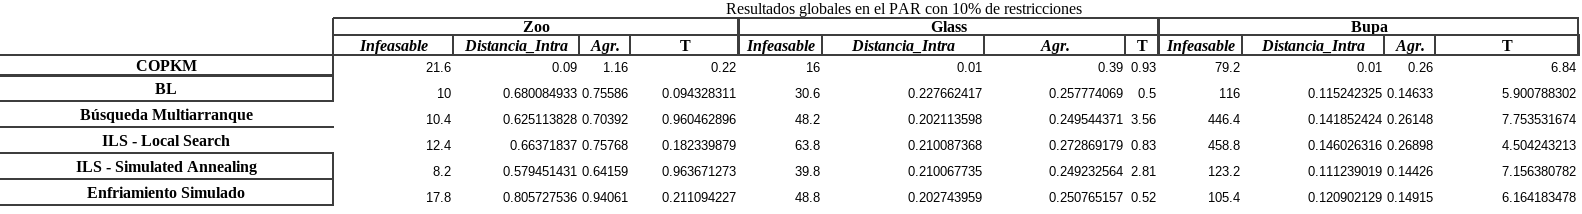
\includegraphics[width=1.0\textwidth]{tablas_globales_10}
    \caption{Tablas Globales - 10\% de restricciones}
\end{figure}

\begin{figure}[H]
    \centering
    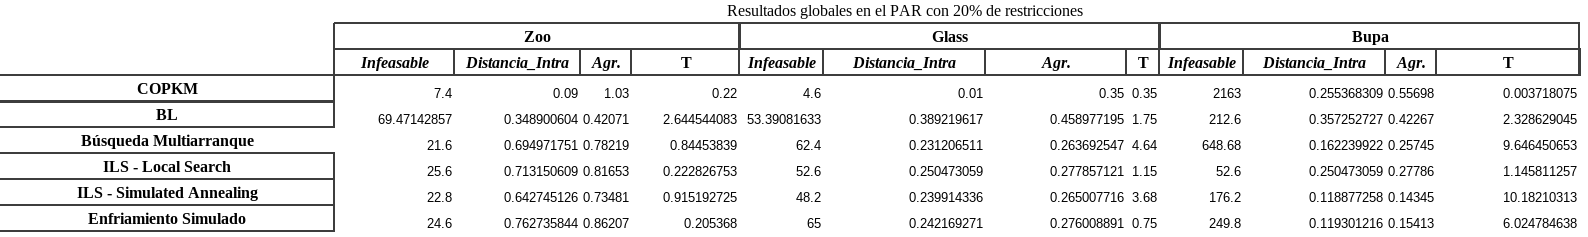
\includegraphics[width=1.0\textwidth]{tablas_globales_20}
    \caption{Tablas Globales - 20\% de restricciones}
\end{figure}

\subsection{Análisis de resultados}

\subsubsection{Análisis general de los resultados}

Para este análisis va a resultar muy útil tener en cuenta los algoritmos que mejor y peor resultado han dado en cada uno de los casos del problema:

\begin{figure}[H]
    \centering
    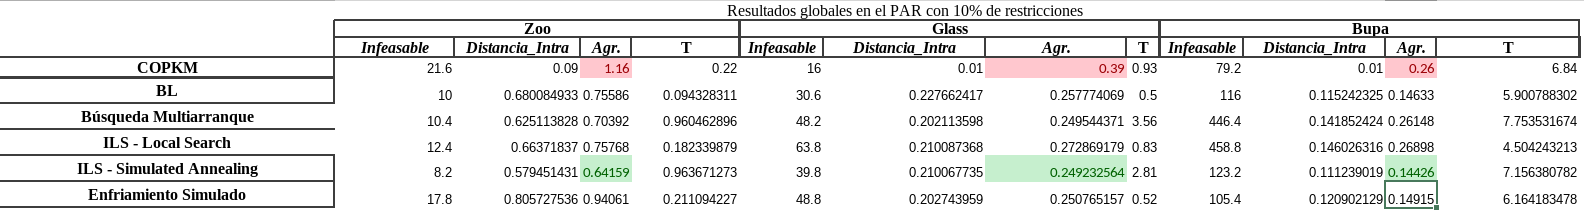
\includegraphics[width=1.0\textwidth]{tablas_mejor_peor_10}
    \caption{Mejor y peor algoritmo, 10\% de las restricciones}
\end{figure}

\begin{figure}[H]
    \centering
    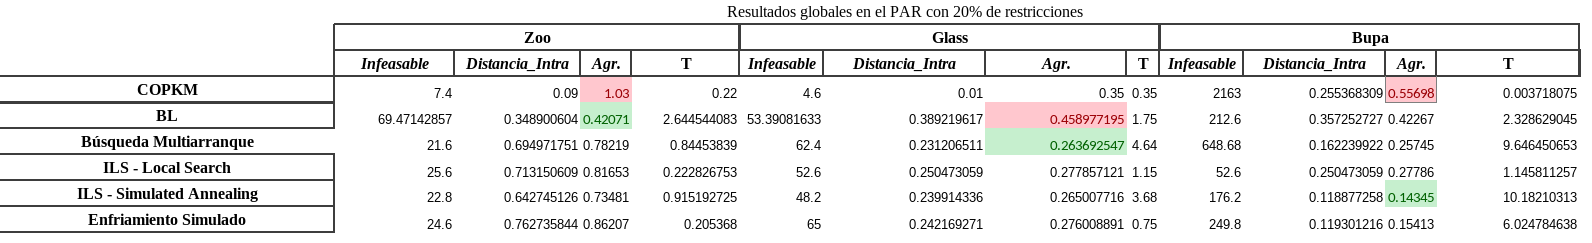
\includegraphics[width=1.0\textwidth]{tablas_mejor_peor_20}
    \caption{Mejor y peor algoritmo, 20\% de las restricciones}
\end{figure}

Como no hemos modificado ni corregido nada respecto de la práctica anterior, los resultados de la búsqueda local y búsqueda \emph{copkmeans} son los mismos que en la práctica anterior.

Fijándonos en los resultados en los \emph{datasets} con el 10\% de las restricciones, cabe destacar que el peor algoritmo siempre ha sido \emph{copkmeans}. Por tanto, los nuevos algoritmos introducidos en esta práctica han tenido un comportamiento como mínimo decente sobre estos conjuntos con el 10\% de las restricciones. Recordar que en la práctica anterior, algunos de los algoritmos tenían un comportamiento nefasto según la configuración del problema, obteniendo resultados peores que \emph{copkmeans}. Y en los tres problemas con el 10\% de los resultados, el mejor algoritmo ha sido \emph{ILS-Enfriamiento Simulado}.

Esto puede ser porque, a pesar de que la intensificación usando enfriamiento simulado sea menos inteligente que la intensificación con búsqueda local, en muchas ocasiones sea útil salir de óptimos locales. Sobre todo en repeticiones tardías de la búsqueda iterativa, donde la intensificación por búsqueda local puede desperdiciar muchas evaluaciones del fitness al quedar atascada en óptimos locales demasiado rápido. Además, la búsqueda con enfriamiento acepta resultados peores con mayor probabilidad al principio, luego en iteraciones más tardías de la intensificación acabaremos con un comportamiento más o menos similar a la búsqueda local.

En los conjuntos con el 20\% de las restricciones tenemos algo más de variedad. Se sigue manteniendo el hecho de que en ninguno de los casos los nuevos algoritmos sean peores que \emph{copkmeans}. Solo en \emph{Glass} la búsqueda local es peor que \emph{Copkmeans}. Y en ese caso, los cuatro algoritmos restantes siguen siendo mejores que \emph{copkmeans}.

En el caso de \emph{Zoo} el mejor algoritmo es la búsqueda local. Esto puede venir motivado porque, al no tener que repartir las evaluaciones entre 10 repeticiones distintas, tenemos 10 veces más iteraciones para intensificar. Con lo que, si no caemos en malos óptimos locales, es lógico pensar que vamos a encontrar mejores soluciones. Esta es la explicación mas sensata a lo que ha pasado en este caso concreto.

La búsqueda local multiarranque ha sido la ganadora en el caso de \emph{Glass}, seguida en segundo lugar de \emph{ILS-Enfriamiento Simulado}. No es sorprendente, pues enfriamiento simulado es una búsqueda menos inteligente que la búsqueda local el primero mejor.

En el caso de \emph{Bupa}, vuelve a ganar \emph{ILS-Enfriamiento Simulado}, seguido por enfriamiento simulado. Con esta configuración de tamaño funcionan muy bien las técnicas basadas en el enfriamiento simulado, el permitir soluciones peores ha sido clave para este problema. Esto se puede ver también el \emph{Bupa 10\%} donde hemos acabado en la misma situación que en este caso.

Todos los algoritmos han tenido comportamientos decentes. El único que no ha destacado en ningún momento ha sido la búsqueda local iterativa usando como intensificador la búsqueda local, obteniendo consistentemente resultados mediocres. El enfriamiento simulado tampoco ha sido el mejor nunca, pero en las dos variantes del problema \emph{Bupa} ha tenido resultados muy buenos, parecidos a los que obtuvo \emph{ILS-Enfriamiento Simulado}, cayendo en la segunda posición. Este comportamiento puede ser debido a lo que en parte ya hemos comentado. En repeticiones tardías de la búsqueda iterativa, a pesar de la fuerte mutación, la intensificación por búsqueda local puede caer en un mal óptimo demasiado rápido, desperdiciando muchas evaluaciones del fitness sin consumir en esa repetición.

Una mejora a este mal comportamiento de \emph{ILS-Local Search} podría ser repetir hasta consumir las evaluaciones del fitness, no hasta un número prefijado de iteraciones. Con ello, si el problema de este algoritmo es efectivamente el que hemos comentado, tendría un menor impacto en el rendimiento del algoritmo.

Cabe destacar los buenos resultados que hemos obtenido con unos algoritmos que han sido muy rápidos de programar. Una vez que hemos programado la búsqueda local, el enfriamiento simulado y los operadores auxiliares, programar estos métodos ha sido muy sencillo, requiriendo muy poco esfuerzo de ingeniería. Por tanto, una vez hecha la base de código que ya hemos comentado, parece sensato siempre probar con estas variantes que son muy sencillas de introducir y mejoran los resultados. Y entre estos, el más destacable es la búsqueda local multiarranque, que prácticamente no ha supuesto esfuerzo de implementación.

En resumen de este primer análisis, el algoritmo que se ha impuesto sobre el resto ha sido \emph{ILS-Enfriamiento simulado}. El resto de los algoritmos han tenido un comportamiento decente, siendo la búsqueda local iterativa con búsqueda local como intensificador el único con resultados mediocres.

Respecto a los tiempos de ejecución no hay demasiado que comentar. En media, el algoritmo que más ha tardado en ejecutarse ha tomado poco más de 10 segundos en \emph{Bupa}. En los problemas con el 10\% de las restricciones, el más lento ha sido \emph{ILS-Enfriamiento Simulado}. En los problemas con el 20\% de las restricciones, los más lentos han sido búsqueda local multiarranque e \emph{ILS-Enfriamiento Simulado}. Sin embargo, no han diferido en distintos órdenes de magnitud, por lo tanto, no parece relevante realizar un análisis de estas diferencias de tiempo. Factores difíciles de capturar, como los cambios de contexto que realizamos en nuestro código, optimizaciones del compilador o fallos de caché pueden ser los causantes de estas diferencias, viendo lo parecidos que son los tiempos de ejecución.

\subsubsection{Algunas comparaciones}

La comparación más directa es la de búsqueda local con búsqueda local multiarranque. La búsqueda local tiene la bondad de que emplea todas las evaluaciones en un único proceso de búsqueda, por lo que, si no cae en óptimos locales de mala calidad, tiene 10 veces más evaluaciones del fitness para intensificar más la solución. Por el otro lado, la búsqueda local multiarranque tiene 10 veces menos evaluaciones del fitness, pero las 10 repeticiones debieran dar mucha más estabilidad y robustez.

En los conjuntos con 10\% de restricciones, solo en \emph{Bupa} la búsqueda local es mejor. Esto tiene sentido, pues es un problema más grande en el que pueden ser necesarias más iteraciones de las que otorgamos a cada una de las búsquedas en la búsqueda multiarranque. En los conjuntos con el 20\% de las restricciones tan solo en \emph{Zoo} la búsqueda local le gana a la búsqueda local multiarranque. De hecho, en \emph{Glass} el peor algoritmo es la búsqueda local y el mejor es la búsqueda local multiarranque.

Mostramos las desviaciones típicas para justificar lo que hemos comentado sobre la robustez:

\begin{figure}[H]
    \centering
    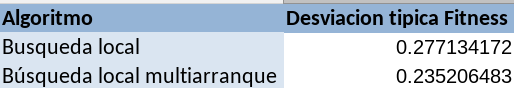
\includegraphics[width=0.5\textwidth]{desviaciones}
    \caption{Desviaciones en el \emph{fitness} de la búsqueda local y \emph{BLM}}
\end{figure}

Por tanto, argumentamos estadísticamente que la búsqueda local es más sensible a la semilla aleatoria respecto al \emph{fitness} de la solución obtenida que la búsqueda local multiarranque, pues su desviación típica es menor.

Ya hemos comparado la búsqueda local iterativa en sus dos variantes, concluyendo que el mejor comportamiento lo otorga el uso de enfriamiento simulado como intensificador. Esto, de nuevo, creemos que es porque la búsqueda local cae demasiado rápido en óptimos locales, desperdiciando evaluaciones del fitness sin consumir.

\subsubsection{Posibles mejoras}

Como ya hemos comentado, sería interesante que, en las búsquedas iterativas, en vez de fijar el parámetro de repeticiones, repitiésemos hasta agotar las evaluaciones del fitness, previo fijado del máximo de evaluaciones en cada intensificación. Con esto seguramente \emph{ILS-Búsqueda local} habría sido más competitivo.

Por otro lado, en enfriamiento simulado, hemos dejado fijo el valor $k = 1$. Podría haber sido interesante realizar algún proceso de búsqueda como \emph{grid search} para fijar un mejor valor de dicho parámetro $k$.

\pagebreak

% Referencias bibliográficas
\bibliography{References}
\bibliographystyle{ieeetr}


\end{document}
